\chapter{Flash Memory Background} \label{sec:flashbackground}

This section provides background material on Flash memory and
its operating principles to aid understanding of our Flash-based
information hiding scheme.

\section{Floating Gate Transistors}

Flash memory is composed of arrays of floating-gate transistors.
A floating-gate transistor is a transistor with two gates,
stacked on top of each other. One gate is electrically insulated
(floating). Figure~\ref{fig:fgtrans} shows an example of a floating-gate device.
The control gate is on top. An insulated conductor, surrounded
by oxide, is between the control gate and the channel. This
conductor is the floating gate. Information is stored as the
presence or absence of trapped charge on the floating gate. The
trapped negative charge reduces the current flowing through the
channel when the N-type MOS transistor is on. This current
difference is sensed and translated into the appropriate binary
value.


\begin{figure} 
\begin{center} 
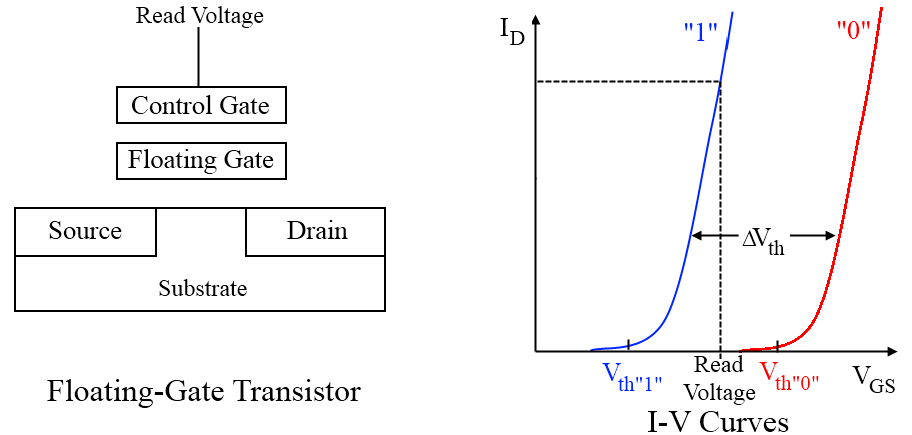
\includegraphics[width=\mywidth]{figs/fgtrans-cleanaxis.png} 
%\includegraphics[width=3.0in]{figs/eval_performance_diff_context.pdf} 
\caption{Flash memory cell based on a floating gate transistor.}
\label{fig:fgtrans} 
%\vspace{-0.25in}
\end{center} 
\end{figure} 

Flash cells without charge on their floating-gate allow full
current flow in the channel and hence are read as a binary ``1''.
The presence of charge on the floating-gate will discourage the
presence of current in the channel, making the cell store a ``0''.
Effectively, the charge on the floating-gate increases the
threshold voltage (Vth) of a transistor. Single-level cells (SLC)
store one bit of information per cell by using two threshold
voltage levels.
Multi-level cells (MLC) store more than one bit by more finely
dividing the threshold voltage levels: for example, four levels 
can be used to store two bits per cell.

%Note that the threshold voltage without any charge on the
%floating-gate is different for each transistor due to variations
%in %manufacturing processes. As a result, the amount of charge
%that needs to be stored to the floating-gate for a cell to
%reliably represent a %''0'' state varies from cell to cell. If
%the threshold voltage is not shifted sufficiently, a cell can be
%in an unreliable (partially %programmed) state that can be
%interpreted as either 1 or 0. In this paper, we exploit the
%threshold voltage variations and the partially %programmed state
%to hide and later to read hidden information.

\section{Flash Organization and Operation}

At a high-level, Flash memory provides three major operations:
read, erase, and program (write). In order to read a bit in a
Flash cell, the corresponding transistor is turned on and the
amount of current is detected. A write to a Flash cell involves
two steps. First, an erase operation pushes charge off the
floating-gate by applying a large negative voltage on the
control gate. Then, a program (write) operation stores charge on
the floating-gate by selectively applying a large positive
voltage if the bit needs to be zero.

An important concept in Flash memory operation is that of pages
and blocks. Pages are the smallest unit in which data is read or
written, and are usually 2KB to 8KB. Blocks are the smallest
unit for an erase operation and made up of several pages,
usually 32 - 128 pages. Note that Flash does not provide
bit-level program or erase. To read an address from a Flash
chip, the page containing the address is read. To update a
value, the block that includes the address must be first erased.
Then, the corresponding page is written with an update and other
pages in the block are restored.

\section{Aging} 

Flash requires high voltages to store and erase information.
The voltages involved place great stress on the device oxide;
each program operation and each erase operation slightly damages the oxide,
wearing out the device.
After thousands of program and erase cycles, the oxide could
have sustained enough damage to render the bit non-operational, leaving
it in a stuck-at state or in a leaky state that cannot reliably 
hold information over a period of time. Flash is usually
guaranteed by the manufacturer up to a certain number of program
and erase cycles. 

Even before failures, the stress causes
the cell's analog characteristics to change. In particular, the
program time that is required to flip a state from '1' to '0' for
a cell tends to reduce as the number of program/erase (PE) cycles increases
for that cell. We exploit this program time shift in order to
hide information.



\section{Partial Programming}

Our information hiding scheme relies on the measurement of program
time, the time it takes to program a Flash cell, at individual cell
granularity. However, the standard Flash memory interface
requires all bits in a page to be programmed together. 
Normally, a program operation on a page is held for a long enough time 
that any cell level variation within a page is overcome. 
Therefore, the normal program time only reveals how long programming
the entire page takes, not how long it takes to program individual bits.

To find the program time on a per-cell basis, we use
a technique called ``partial programming'' \cite{flash-ieeesp2012}.
The standard Flash memory interfaces allow the ``partial program'' 
of a cell by aborting a program operation before completion. 
If the program
operation is interrupted, the Flash cell may be in an unreliable
state that could be interpreted as 1 or 0. Further ``partial
programs'' will accumulate charge on the floating gate and
eventually result in the cell entering a stable programmed
state, as if a full program was applied. Effectively, the number of
partial program operations to flip a bit from 1 to 0 represents
the program time for the bit.
In this sense, we use the ``partial programming'' technique to 
to find program time for individual cells. After a partial program to a
page, we read the page and record the state of each bit. When a
bit changes to the programmed state (from 1 to 0), we
note the number of partial programs required to flip the bit as 
the bit's program time.

